\chapter{MATERYAL VE YÖNTEM}



% Basit iki terimle \acrfull{OBEB} ve \acrfull{OKEK} kısaltmaları anlatabiliriz. İster kısaltmasını \acrshort{OBEB}, isterseniz de uzun açılımını \acrlong{OKEK} yazdırabilirsiniz. Bunu yapabilmek için dosyanın başında terimleri tanımlamanız gereklidir. İsterseniz matematik terimlerini de, örneğin \acrshort{pi} böyle tanımlayabilirsiniz. Uzun uzun \acrfull{pi} yazmanız gerekmez. 

% Teorem yazmak isterseniz:
% \begin{theorem}[Öklid]
%  İki noktadan bir ve yalnız bir doğru geçer.
% \end{theorem}

% İspat yazmak isterseniz:
% \begin{ispat}[Tezin en önemli ispatı]
% x=10
% \end{ispat}
% \lipsum[1-2]
% \begin{figure}[h]
% \centering
% 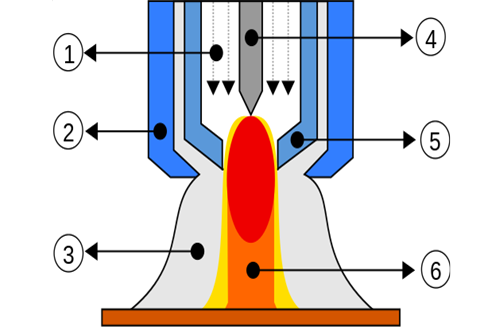
\includegraphics[width=\textwidth]{gorseller/ptaTorc}
% \caption{PTA Torç}\label{fig:PtaTorc1}
% \end{figure}
% \lipsum[1-2]
% \begin{table}
% \centering
% \caption{Deneme Tablosu.}\label{tab:den1}
% \begin{tabular}{|l|l|l|}
% \hline
% sıra   & sayı   & toplam \\ \hline
% 1      & 2      & 3      \\ \hline
% Kelime & deneme & son    \\ \hline
% \end{tabular}
% \end{table}


\section{Veri Kümesi}


\subsection{Haple Pasite Caseto Harra veri kümesi}
% \lipsum[1-2]
% \begin{table}[!bp]
% \centering
% \caption{CK+ veri setindeki her sınıf için örnek sayısı}
% \label{tab:datasetclasses}
% \begin{tabular}{|l|l|l|}
% \hline
% sıra   & sayı   & toplam \\ \hline
% 1      & 2      & 3      \\ \hline
% Kelime & deneme & son    \\ \hline
% \end{tabular}
% \end{table}


\lipsum[5-6]

\begin{figure}[ht]
\centering
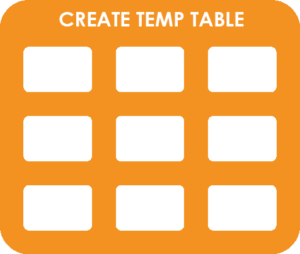
\includegraphics[width=0.99\textwidth]{gorseller/Temporary-Table.PNG}
\caption{wsdwwww}\label{fig:ckexample}
\end{figure}

\lipsum[6]. Çizelge\ref{tab:datasetclasses}'de.


\begin{table}[ht]
	\centering
	\tabulinesep=1mm
	\caption{Haple Pasite Caseto Harra veri kümesindeki her sınıf için örnek sayısı}
	\vspace{15mm}
	\newcommand{\tablecolumnsize}{0.075\columnwidth}
	
	{\normalsize 
		\begin{tabu} {
				>{\centering}m{\tablecolumnsize}
				>{\centering}m{\tablecolumnsize}
				>{\centering}m{\tablecolumnsize}
				>{\centering}m{\tablecolumnsize}
				>{\centering}m{\tablecolumnsize}
				>{\centering}m{\tablecolumnsize}
				>{\centering}m{\tablecolumnsize}
				>{\centering}m{\tablecolumnsize}
			}
			\begin{rotate}{45} sub1 \end{rotate} &
			\begin{rotate}{45} sub2 \end{rotate} &
			\begin{rotate}{45} sub3 \end{rotate} &
			\begin{rotate}{45} sub4 \end{rotate} &
			\begin{rotate}{45} sub5 \end{rotate} &
			\begin{rotate}{45} sub6 \end{rotate} &
			\begin{rotate}{45} sub7 \end{rotate} &
			\begin{rotate}{45} \textbf{Toplam} \end{rotate} \\
			\tabucline[1.5pt]{-}
			901 & 82 & 1582 & 121 & 1328 & 111 & 321 & \textbf{4122}
		\end{tabu}
	}
	
	\label{tab:datasetclasses}
\end{table}

\subsection{OPLE Cople Gubele Heo port}

\lipsum[19]
yöntem \parencite{Chawla_2002} 
\lipsum[16]
Çizelge-\ref{tab:smotetablo}'de verilmiştir. 

\begin{table}
\centering
\caption{Veri kümesindeki vektor sayıları}\label{tab:smotetablo}
\begin{tabular}{|l|l|l|}
\hline
\textbf{Sınıf}   & \textbf{Veri1}   & \textbf{Veri2} \\ \hline
sub1      & 231    & 355      \\ \hline
sub2 & 822 & 355    \\ \hline
sub3 & 165 & 355    \\ \hline
sub4 & 452 & 355    \\ \hline
sub5 & 312 & 355    \\ \hline
sub6 & 122 & 355    \\ \hline
sub7 & 322 & 355    \\ \hline
Toplam & 3135 & 3135    \\ \hline
\end{tabular}
\end{table}

% \begin{table}[ht]
% 	\centering
% 	\tabulinesep=1mm
% 	\caption{CK+ Veri Kümesi için SAAÖT Algoritması Uygulandığındaki Örnek Dağılımı}
% 	\vspace{10mm}
% 	\newcommand{\tablecolumnsize}{0.075\columnwidth}
	
% 	{\normalsize 
% 		\begin{tabu} {
% 				>{\centering}m{\tablecolumnsize}
% 				>{\centering}m{\tablecolumnsize}
% 				>{\centering}m{\tablecolumnsize}
% 				>{\centering}m{\tablecolumnsize}
% 				>{\centering}m{\tablecolumnsize}
% 				>{\centering}m{\tablecolumnsize}
% 				>{\centering}m{\tablecolumnsize}
% 				>{\centering}m{\tablecolumnsize}
% 			}
% 			\begin{rotate}{45} Öfke \end{rotate} &
% 			\begin{rotate}{45} Küçümseme \end{rotate} &
% 			\begin{rotate}{45} İğrenme \end{rotate} &
% 			\begin{rotate}{45} Korku \end{rotate} &
% 			\begin{rotate}{45} Mutluluk \end{rotate} &
% 			\begin{rotate}{45} Üzüntü \end{rotate} &
% 			\begin{rotate}{45} Şaşırma \end{rotate} &
% 			\begin{rotate}{45} \textbf{Toplam} \end{rotate} \\
% 			\tabucline[1.5pt]{-}
% 			166 & 166 & 166 & 166 & 166 & 166 & 166 & \textbf{1162}
% 		\end{tabu}
% 	}
	
% 	\label{tab:smoteclasses}
% \end{table}

% \subsection{Bulgular ve Tartışma ikinci derece başlık}
% \lipsum[1-2]
% \begin{figure}[h]
% \centering
% 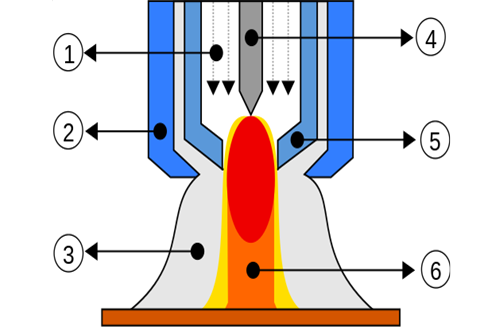
\includegraphics[width=\textwidth]{gorseller/ptaTorc}
% \caption{PTA Torç}\label{fig:PtaTorc1}
% \end{figure}
% \lipsum[1-2]
% \begin{table}
% \centering
% \caption{Deneme Tablosu.}\label{tab:den1}
% \begin{tabular}{|l|l|l|}
% \hline
% sıra   & sayı   & toplam \\ \hline
% 1      & 2      & 3      \\ \hline
% Kelime & deneme & son    \\ \hline
% \end{tabular}
% \end{table}

% Teorem yazmak isterseniz:
% \begin{theorem}[Öklid]
%  İki noktadan bir ve yalnız bir doğru geçer.
% \end{theorem}

% İspat yazmak isterseniz:
% \begin{ispat}[Tezin en önemli ispatı]
% x=10
% \end{ispat}

% \subsubsection{Bulgular ve tartışma dördüncü derece başlık}
% \lipsum[1-2]
% \begin{figure}[h]
% \centering
% 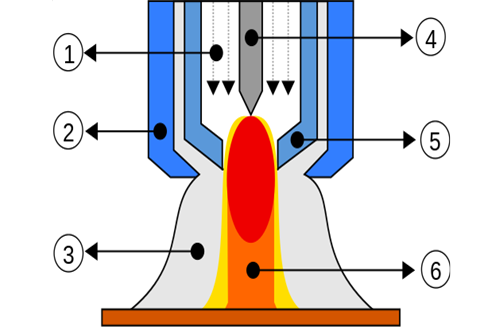
\includegraphics[width=\textwidth]{gorseller/ptaTorc}
% \caption{PTA Torç}\label{fig:PtaTorc1}
% \end{figure}
% \lipsum[1-2]
% \begin{table}
% \centering
% \caption{Deneme Tablosu.}\label{tab:den1}
% \begin{tabular}{|l|l|l|}
% \hline
% sıra   & sayı   & toplam \\ \hline
% 1      & 2      & 3      \\ \hline
% Kelime & deneme & son    \\ \hline
% \end{tabular}
% \end{table}

% Teorem yazmak isterseniz:
% \begin{theorem}[Öklid]
%  İki noktadan bir ve yalnız bir doğru geçer.
% \end{theorem}

% İspat yazmak isterseniz:
% \begin{ispat}[Tezin en önemli ispatı]
% x=10
% \end{ispat}
% Eğer metin içinde \(\lim_{x \to \infty} \exp(-x) = 0\) ya da ortalayabilir
% \begin{displaymath}
% \cos (2\theta) = \cos^2 \theta - \sin^2 \theta
% \end{displaymath}
% isterseniz de numaralı denklem yazabilirsiniz.

% \begin{equation}
% \frac{\mathrm d}{\mathrm d x} \left( k g(x) \right)
% \end{equation}
% \subsubsection{Kimya}
% \ce{B4C} yazabilirsiniz. Ya da

% \ce{CO2 + C -> 2CO}

% Daha fazlası için mhchem paketine bakınız.
 
% Eğer metin içinde şekile referans vermek isterseniz Şekil\ref{fig:68point} yazarsınız. 

% Kaynakça böyle verilebilir \parencite{celik_microstructure_2013} ya da iki yazarlı ise böyle verilebilir \parencite{gatto_plasma_2004} veya ikiden fazla ise böyle verilebilir.
% \parencite{celik_effects_2011}

% Kaynakça listesi için daha çok referans verilmek istenirse \parencite{yazdi_microstructure_2015, keehan_influence_2006, guo_microstructure_2014}, \parencite{kim_variation_2013}, bir başkası \parencite{xibao_metallurgical_2005},  ya da başkası \parencite{jin_effect_1997} kullanılabilir.

\section{Yöntem}


\lipsum[14-16]
\acrshort{lbp} \acrshort{hog} .


\lipsum[18-20] Şekil-\ref{fig:flowchart} da verilmiştir.


\begin{figure}[hp]
\centering

\begin{tikzpicture}[node distance=2cm]

\node (start) [startstop] {Başlama};
\node (in1) [io, below of=start] {start};
\node (pro1) [process, below of=in1] {forward1};
\node (pro2) [process, below of=pro1] {forward2};
\node (dec1) [decision, below of=pro2, yshift=-2.5cm] {opt};

\node (pro3) [process, below of=dec1, yshift=-2.0cm] {opt2};
\node (out1) [io, below of=pro3] {final};
\node (stop) [startstop, below of=out1] {finish};

\coordinate (point1) at (-4cm,-4.2cm);
\coordinate (point2) at (-1.7cm,-4.2cm);
\coordinate (point3) at (-2.5cm,-10.5cm); 

\draw [arrow] (start) -- (in1);
\draw [arrow] (in1) -- (pro1);
\draw [arrow] (pro1) -- (pro2);
\draw [arrow] (pro2) -- (dec1);
\draw [arrow] (dec1) -- node[anchor=east] { } (pro3);
\draw [] (point2) -- (point1);
\draw [arrow] (point1) |- (dec1);
\draw [arrow] (pro3) -- (out1);
\draw [arrow] (out1) -- (stop);

\end{tikzpicture}
\caption{Akış diyagramı}\label{fig:flowchart}
\end{figure}

